% algorithmes de flot max

\begin{frame}{Le problème du flot maximal}
    \begin{itemize}
        \item Capacité de transport : réseaux de trains, de canalisation, câbles électriques, réseaux d'information, réseaux routiers, infrastructures de transport multimodales\dots
        \item La question : combien (d'information, d'eau, de touristes, de voitures,  d'élections\dots) peut-on faire transiter sur ce réseau ?
        \item Formalisation : faire passer la plus grande quantité de matière entre une source $s$ et une destination $t$. Les liens permettant d'acheminer le flux ont une \emph{capacité} limitée et il n'y a ni perte ni création de matière lors de l'acheminement 
        \item On se donne 
        \begin{itemize}
            \item un graphe orienté $G=(S,A)$
            \item une fonction de capacité $c : A \longrightarrow \nbR^+$
            \item 2 sommets particuliers de $S$ : $s$ et $t$ 
        \end{itemize}
    \end{itemize}
\end{frame}

\begin{frame}{Problème du flot maximal}
    \begin{definition}
        Un \emph{flot} est une fonction $f : A \longrightarrow \nbR^+$ telle que 
        \begin{itemize}
            \item $0 \leq f(a) \leq c(a), \forall a \in A$ (contrainte de capacité)
            \item $ \sum_{(i,j) \in A} f(i,j) = \sum_{(j,k) \in A} f(j,k) \forall j \neq s,t$ (contrainte de conservation)
        \end{itemize}
    \end{definition}
    \begin{itemize}
        \item Pour vérifier la loi de conservation en tous sommets, on va ajouter au graphe un arc de retour fictif entre $t$ et $s$ et on appellera \emph{valeur du flot} $val(f)$ la quantité $f(t,s)$ 
        \item On cherche alors à maximiser $val(f)$ 
        \item NB : c'est un programme linéaire sous contraintes !
    \end{itemize}
\end{frame}

\begin{frame}{Représentation graphique}
    \begin{center}
        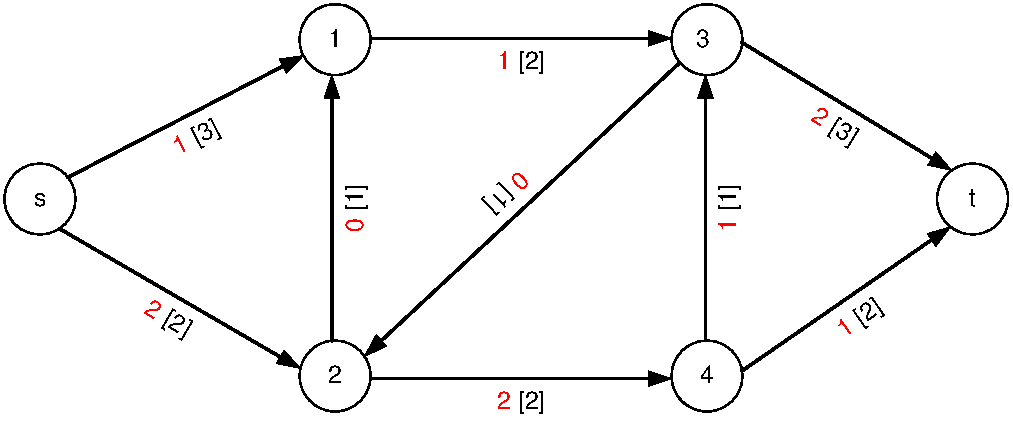
\includegraphics[height=.5\textheight]{fig/flot1.pdf}
    \end{center}
    Convention : la capacité est représentée entre crochets 
\end{frame}

\begin{frame}{Représentation graphique avec arc de retour fictif}
    \begin{center}
        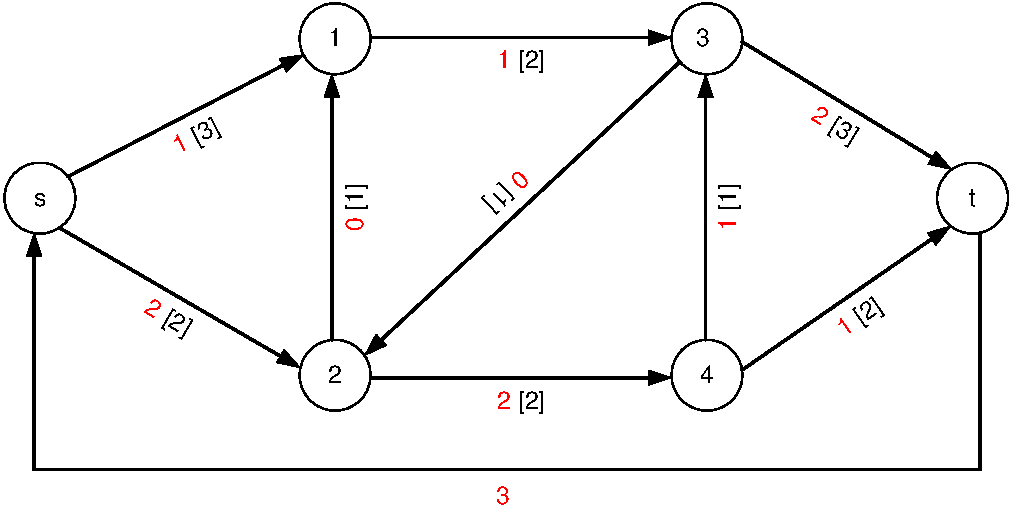
\includegraphics[height=.5\textheight]{fig/flot2.pdf}
    \end{center}
\end{frame}

\begin{frame}{Algorithme de Ford-Fulkerson}
    \begin{itemize}
        \item Principe 
        \begin{itemize}
            \item Le flot nul est toujours réalisable : point de départ
            \item Idée : si on trouve d'un chemin d'arcs non saturés de $s$ à $t$, alors on peut augmenter le flot le long de ce chemin 
        \end{itemize}
        \item pour un flot donné, capacité résiduelle d'un arc $a$ : $c^r(a) = c(a) - f(a)$
        \item on dit qu'un arc est saturé si sa capacité résiduelle est nulle, $c^r(a) = 0$
        \item \textbf{Mais cette notion n'est pas toujours suffisante !}
        \begin{itemize}
            \item en clair, risque de minimum local 
        \end{itemize}
    \end{itemize}
\end{frame}

\begin{frame}{Chaine augmentante}
    \begin{definition}
        Une chaine augmentante de $s$ à $t$ pour un flot admissible donné est une chaine respectant les contraintes suivantes :
        \begin{itemize}
            \item $f(a) < c(a)$ pour tout arc $a$ dirigé de $s$ vers $t$ 
            \item $f(a) > 0$ pour tout arc dirigé de $t$ vers $s$
        \end{itemize}
    \end{definition}    
    \begin{example}
        \begin{center}
            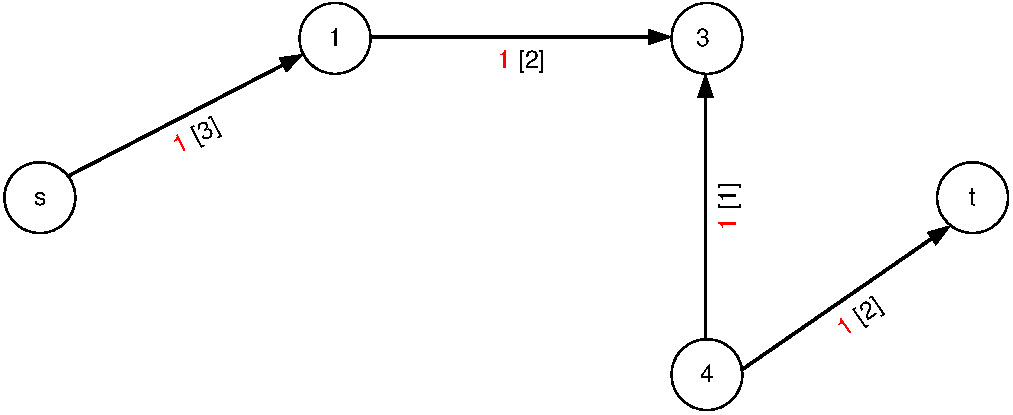
\includegraphics[height=0.35\textheight]{fig/flot3.pdf}
        \end{center}
        
    \end{example}
\end{frame}

\begin{frame}{Augmentation du flot le long d'une chaine augmentante}
    \begin{itemize}
        \item Le flot peut alors être augmentée d'une quantité $\alpha$ définie par 
        $$
        \alpha = \min \left[ 
            min_{a \in \mu^+} (c(a) - f(a)) , \min_{a \in \mu^- } f(a)
        \right]
        $$
        \item où $\mu^+$ (respectivement $\mu^-$) est l'ensemble des arcs orientés de $s$ vers $t$ dans la chaine (respectivement de $t$ vers $s$)
        \item On peut alors augmenter le flot de $\alpha$ sur les arcs de  $\mu^+$ et le diminuer de $\alpha$ sur les arcs de $\mu^-$
    \end{itemize}
\end{frame}

\begin{frame}{Coupes}
    \begin{definition}
        Une st-coupe associée à un graphe $G=(X,A)$ est une partition de $X$ en deux ensembles $S$ et $T$ tels que $s \in S$ et $t \in T$. 
        
        On appelle capacité de cette st-coupe $c(S,T) = \sum_{i \in S, j \in T} c(i,j)$ 
    \end{definition}
    \begin{theorem}
        Un flot de $s$ à $t$ est maximal s'il n'existe pas de chaine augmentante de $s$ à $t$.
    \end{theorem}
    \begin{block}{Corollaire}
        Quelle que soit la st-coupe $(S,T)$, quel que soit le flot $f$, la valeur du flot $val(f)$ est inférieure ou égale à la capacité de cette coupe : $val(f) \leq c(S,T)$.
    \end{block}
\end{frame}

\begin{frame}{Théorème de Ford-Fulkerson}
    \begin{theorem}
        La valeur du flot maximal est égal à la capacité de la coupe minimale 
    \end{theorem}
\end{frame}

\begin{frame}{Schéma de l'algorithme de Ford-Fulkerson}
\label{alg:ford-fulkerson}
    \begin{algorithmic}
        \Function{ff}{(G,s)}
        \State x = (0,...,0) 
        \While{il existe une chaine augmentante de $s$ à $t$} 
            \State $c$ \gets chaine augmentante de $s$ à $t$
            \State $\mu^+$ \gets arcs de $c$ dans le sens $s$ vers $t$ 
            \State $\mu^-$ \gets arcs de $c$ dans le sens $t$ vers $s$
            \State $\alpha = \min \left[ 
                min_{a \in \mu^+} (c(a) - f(a)) , \min_{a \in \mu^- } f(a)
            \right]$
            \For{$a \in \mu^+$} 
                $f(a)$ \gets $f(a)+\alpha$
            \EndFor
            \For{$a \in \mu^-$} 
                $f(a)$ \gets $f(a)-\alpha$
            \EndFor
        \EndWhile
        \EndFunction
    \end{algorithmic}
\end{frame}

\begin{frame}{Déterminer une chaine augmentante}
    \begin{itemize}
        \item Un point n'est pas abordé dans l'algorithme précédent : comment déterminer une chaine augmentante ?
    \end{itemize}
    \begin{definition}
        On appelle \emph{graphe résiduel} $G^r=(S,A^r)$ le graphe associé à une capacité et à un flot donné, avec $\forall a \in A$ :
        \begin{itemize}
            \item si $f(a) < c(a)$ alors on ajoute $a$  $A^R$ avec $c^r(a) = c(a)-f(a)$
            \item si $f(a) > 0$ alors on ajoute $a$ \textbf{en sens inverse} dans $A^r$ avec une capacité égale à $f(a)$
        \end{itemize}
    \end{definition}
    \begin{itemize}
    \item Un parcours en largeur d'abord (BFS) va permettre de trouver l'ensemble des sommets atteignables depuis $s$ dans $G^r$. Si on mémorise pour chaque sommet visité le sommet d'où l'on arrive, on construit ainsi un arbre couvrant. 
    \item On a donc un chemin unique de $s$ à $t$ 
\end{itemize}
\end{frame}


\begin{frame}{Graphe résiduel : exemple}
\begin{center}
    \scalebox{0.65}{\begin{tikzpicture}
\clip (0,0) rectangle (9.0,6.0);
\Vertex[x=0.450,y=3.000,size=0.5,opacity=0.5,label=s]{0}
\Vertex[x=3.150,y=5.700,size=0.5,opacity=0.5,label=A]{1}
\Vertex[x=3.150,y=1.920,size=0.5,opacity=0.5,label=B]{2}
\Vertex[x=3.150,y=0.300,size=0.5,opacity=0.5,label=C]{3}
\Vertex[x=5.850,y=5.700,size=0.5,opacity=0.5,label=D]{4}
\Vertex[x=6.525,y=3.000,size=0.5,opacity=0.5,label=E]{5}
\Vertex[x=5.850,y=0.300,size=0.5,opacity=0.5,label=F]{6}
\Vertex[x=8.550,y=3.000,size=0.5,opacity=0.5,label=t]{7}
\Edge[,lw=1.0,bend=-12.68,label=20 [35],Direct](0)(1)
\Edge[,lw=1.0,bend=-12.68,label=0 [35],Direct](0)(2)
\Edge[,lw=1.0,bend=-12.68,label=0 [40],Direct](0)(3)
\Edge[,lw=1.0,bend=-12.68,label=20 [20],Direct](1)(4)
\Edge[,lw=1.0,bend=-12.68,label=0 [10],Direct](1)(6)
\Edge[,lw=1.0,bend=-12.68,label=0 [15],Direct](2)(4)
\Edge[,lw=1.0,bend=-12.68,label=0 [25],Direct](2)(5)
\Edge[,lw=1.0,bend=-12.68,label=0 [5],Direct](2)(6)
\Edge[,lw=1.0,bend=-12.68,label=0 [20],Direct](3)(5)
\Edge[,lw=1.0,bend=-12.68,label=0 [20],Direct](3)(6)
\Edge[,lw=1.0,bend=-12.68,label=20 [20],Direct](4)(7)
\Edge[,lw=1.0,bend=-12.68,label=0 [30],Direct](5)(7)
\Edge[,lw=1.0,bend=-12.68,label=0 [60],Direct](6)(7)
\end{tikzpicture}
} 
    \scalebox{0.65}{\begin{tikzpicture}
\clip (0,0) rectangle (9.0,6.0);
\Vertex[x=0.450,y=3.000,size=0.5,opacity=0.5,label=s]{0}
\Vertex[x=3.150,y=5.700,size=0.5,opacity=0.5,label=A]{1}
\Vertex[x=3.150,y=1.920,size=0.5,opacity=0.5,label=B]{2}
\Vertex[x=3.150,y=0.300,size=0.5,opacity=0.5,label=C]{3}
\Vertex[x=5.850,y=5.700,size=0.5,opacity=0.5,label=D]{4}
\Vertex[x=6.525,y=3.000,size=0.5,opacity=0.5,label=E]{5}
\Vertex[x=5.850,y=0.300,size=0.5,opacity=0.5,label=F]{6}
\Vertex[x=8.550,y=3.000,size=0.5,opacity=0.5,label=t]{7}
\Edge[fontcolor=green,lw=1.0,bend=-12.68,label=[20],Direct](1)(0)
\Edge[fontcolor=red,lw=1.0,bend=-12.68,label=[15],Direct](0)(1)
\Edge[,lw=1.0,bend=-12.68,label=[35],Direct](0)(2)
\Edge[,lw=1.0,bend=-12.68,label=[40],Direct](0)(3)
\Edge[fontcolor=green,lw=1.0,bend=-12.68,label=[20],Direct](4)(1)
\Edge[,lw=1.0,bend=-12.68,label=[10],Direct](1)(6)
\Edge[,lw=1.0,bend=-12.68,label=[15],Direct](2)(4)
\Edge[,lw=1.0,bend=-12.68,label=[25],Direct](2)(5)
\Edge[,lw=1.0,bend=-12.68,label=[5],Direct](2)(6)
\Edge[,lw=1.0,bend=-12.68,label=[20],Direct](3)(5)
\Edge[,lw=1.0,bend=-12.68,label=[20],Direct](3)(6)
\Edge[fontcolor=green,lw=1.0,bend=-12.68,label=[20],Direct](7)(4)
\Edge[,lw=1.0,bend=-12.68,label=[30],Direct](5)(7)
\Edge[,lw=1.0,bend=-12.68,label=[60],Direct](6)(7)
\end{tikzpicture}
}
\end{center}
\end{frame} 


\directlua{\detokenize{
    for i=0,6,1 do
        tex.sprint("\\begin{frame}{Flot}\\begin{center} \\input{genfig/ff-", i, ".tex} \\end{center} \\end{frame}")
        tex.sprint("\\begin{frame}{Graphe résiduel}\\begin{center} \\input{genfig/ffr-", i, ".tex} \\end{center} \\end{frame}")
    end
}}


\begin{frame}{Choix de la chaine augmentante}
    \begin{itemize}
        \item L'exemple précédent effectue un choix de chaine augmentante, mais n'importe laquelle peut être choisie 
        \item Le flot maximal n'a pas de raison d'être unique
        \item Le choix des chaînes augmentantes influe sur le nombre d'itérations 
    \end{itemize}
    \begin{example}
        \begin{center}
        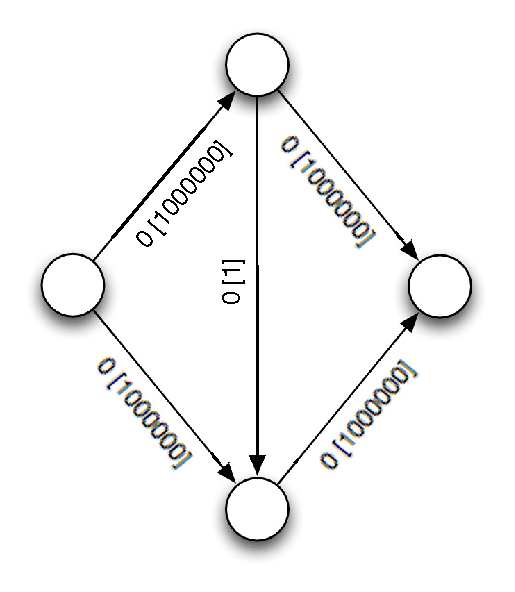
\includegraphics[height=3.5cm]{fig/flotcon-1.pdf}
        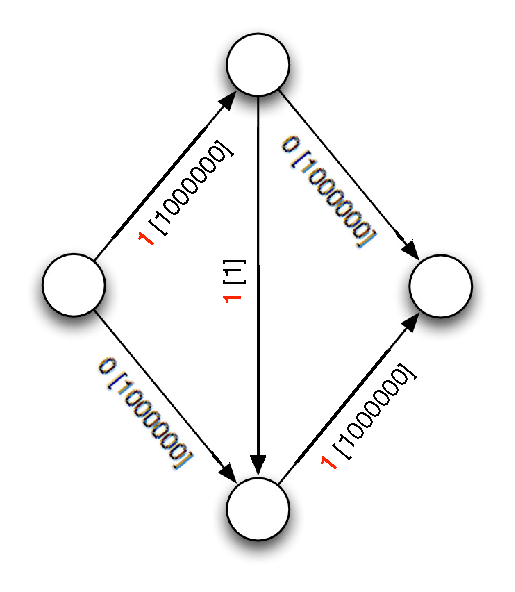
\includegraphics[height=3.5cm]{fig/flotcon-2.pdf}
        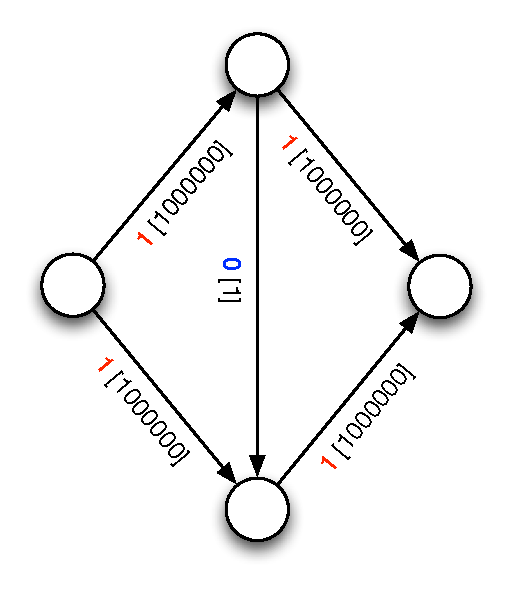
\includegraphics[height=3.5cm]{fig/flotcon-3.pdf}
        \end{center}
    \end{example}
\end{frame}

\begin{frame}{Flot maximal à coût minimal}
    \begin{itemize}
        \item On ajoute une notion de coût unitaire aux graphes utilisés précédemment : $d : A \longrightarrow \nbR^+$
        \begin{itemize}
            \item i.e. le transport d'une quantité $f(a)$ sur un arc $a$ a un coût $d(a)*f(a)$ 
        \end{itemize}
        \item On cherche alors parmi tous les flots maximaux $f$ celui qui minimise $\sum_{a \in A} f(a)d(a)$
        \item 2 approches possibles 
        \begin{itemize}
            \item Partir du flot nul (de coût minimal) et augmenter progressivement le flot (Algorithme de Roy)
            \item Partir d'un flot maximal et en faire diminuer progressivement le coût (Algorithme de Bennington)
        \end{itemize}
    \end{itemize}
\end{frame}


\begin{frame}{Algorithme de Roy}
\label{alg:roy}
\begin{algorithmic}
    \State $x_0 = (0,...,0)$, $k$=0 
    \State Construire le graphe résiduel $G_k^r$
    \While{il existe un chemin de $s$ à $t$ dans $G^r_k$}
        \State Soit $\mu_k$ le plus court chemin de $s$ à $t$ dans $G_k^r$
        \State Soit $c$ la plus petite capacité des arcs de $\mu_k$ 
        \State $$\forall (i,j) \in A, x_{k+1}(i,j) = \left\{ 
            \begin{array}{l}
                x_k(i,j)+c \textrm{ si } (i,j) \in \mu_k \\
                x_k(i,j)-c \textrm{ si } (j,i) \in \mu_k \\
                x_k(i,j) \textrm{ sinon}
            \end{array}
            \right. $$
        \State $k$ \gets $k+1$
    \EndWhile
\end{algorithmic}
\end{frame}

% exemple algorithme de Roy

\begin{frame}{Exemple}
    \begin{center}
        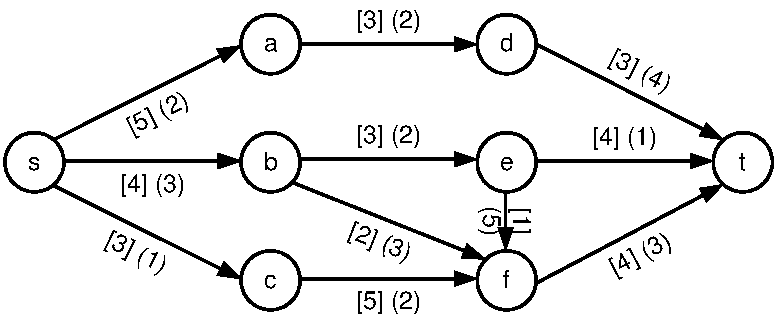
\includegraphics[width=.8\textwidth]{fig/fmcm1.pdf}
    \end{center}
\end{frame}

\begin{frame}{Premier graphe résiduel : le graphe lui-même}
    \begin{center}
        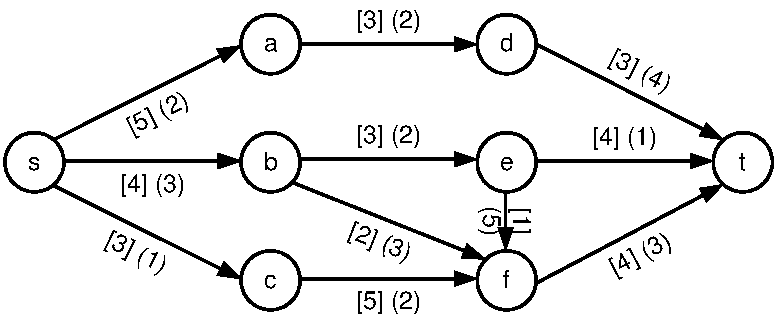
\includegraphics[width=.8\textwidth]{fig/fmcm1.pdf}
    \end{center}

    Plus court chemin : $(s,b,e,t)$ de capacité 3. On augmente le flot de 3.
\end{frame}

\begin{frame}{Second graphe résiduel}
    \begin{center}
        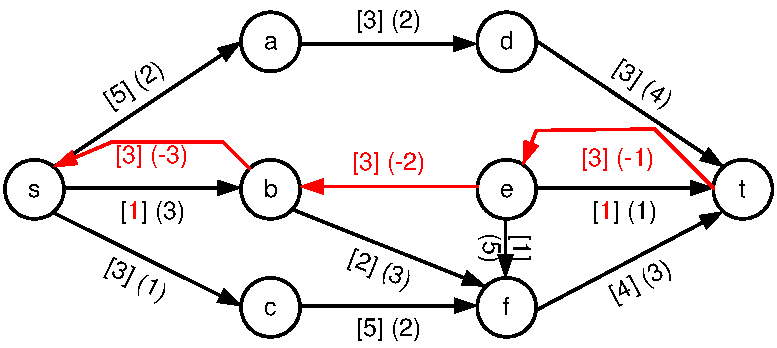
\includegraphics[width=.8\textwidth]{fig/fmcm2.pdf}
    \end{center}

    Plus court chemin : $(s,c,f,t)$ de capacité 3. On augmente le flot de 3.
\end{frame}

\begin{frame}{Troisième graphe résiduel}
    \begin{center}
        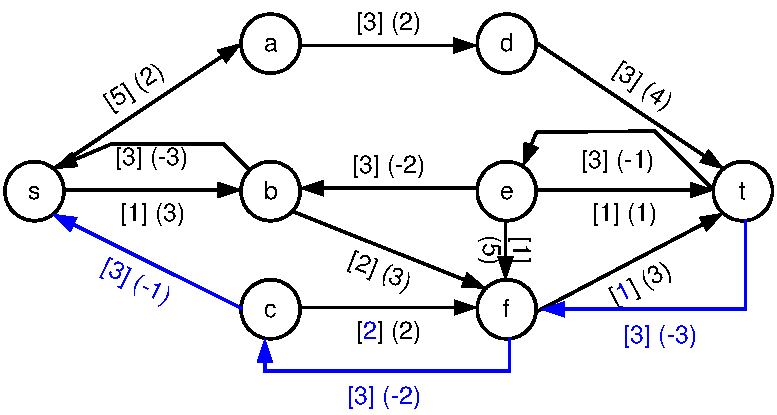
\includegraphics[width=.8\textwidth]{fig/fmcm3.pdf}
    \end{center}

    Plus court chemin : $(s,a,d,t)$ de capacité 3. On augmente le flot de 3.
\end{frame}

\begin{frame}{Quatrième graphe résiduel}
    \begin{center}
        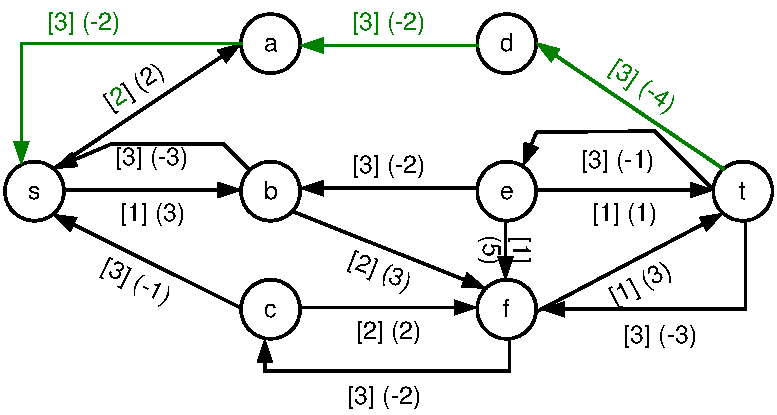
\includegraphics[width=.8\textwidth]{fig/fmcm4.pdf}
    \end{center}

    Plus court chemin : $(s,b,f,t)$ de capacité 1. On augmente le flot de 1.
\end{frame}

\begin{frame}{Cinquième graphe résiduel}
    \begin{center}
        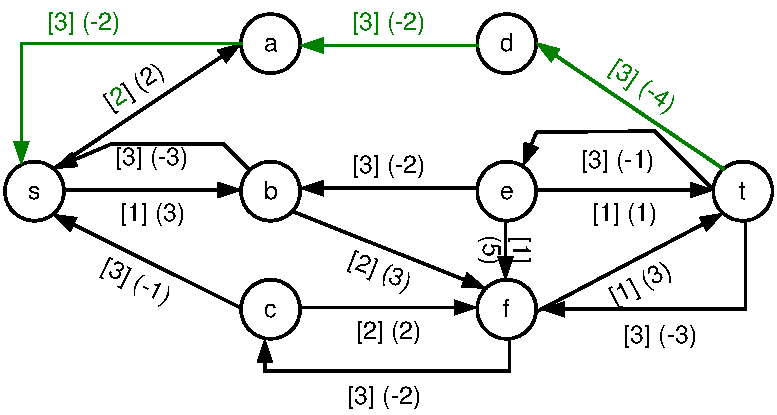
\includegraphics[width=.8\textwidth]{fig/fmcm4.pdf}
    \end{center}

    Pas de chemin entre $s$ et $t$ : l'algorithme est terminé.
\end{frame}





